\documentclass[a4paper]{jpconf}
\usepackage{graphicx}
\begin{document}
\title{Fast emulation of track reconstruction in CMS simulation}

\author{Matthias Komm, on behalf of the CMS collaboration}

\address{Centre for Cosmology, Particle Physics and Phenomenology,
Universit\'e catholique de Louvain, Louvain-la-Neuve, BELGIUM}

\ead{Matthias.Komm@cern.ch}

\begin{abstract}
Simulated samples of various physics processes are a key ingredient within analyses to unlock the physics behind LHC collision data. Samples with more and more statistics are required to keep up with the increasing amounts of recorded data. During sample generation, significant computing time is spent on the reconstruction of charged particle tracks from energy deposits which additionally scales with the pileup conditions. In CMS, the FastSimulation package is developed providing a fast alternative to the standard simulation and reconstruction work flow. It employs various techniques to emulate track reconstruction effects in particle collision events amongst others. Several analysis groups in CMS are utilizing the package, in particular those requiring many samples to scan the parameter space of physics models (e.g. SUSY) or for the purpose of estimating systematic uncertainties. The strategies for and recent developments in this emulation are presented which features a novel, flexible implementation of tracking emulation while retaining a sufficient, tuneable accuracy.
\end{abstract}

\section{Introduction}
Tracking of charged particles is one of the crucial ingredients to understand the physics behind LHC collisions. From reconstructed tracks higher analysis level objects like jets and the missing transverse energy are derived. In the CMS experiment, tracks are utilized even further by matching them to information gathered by other subdetectors improving the overall event reconstruction and resolution.

Sophisticated tracking algorithms are required to reconstruct tracks from the large amount of charged particles transversing the CMS detector at each bunch crossing. A typical instantaneous luminosity of $10^{34}\,\mathrm{cm}^{-2}\mathrm{s}^{-1}$ which was reached in 2016 can lead to more than 500 reconstructed tracks originating from 20--30 proton-proton interactions per event.

The complex, multistep algorithms which reconstruct tracks from energy depositions left by transversing charged particles in the CMS tracker are unsurprisingly very computing-intense. This standard tracking procedure is applied to simulated events as well after those have passed the emulation of the electronic response of the detector. However, at this point in the simulation chain it can be beneficial to sidestep the standard reconstruction by utilizing truth-information about the simulated events instead. In the CMS simulation framework this idea together with others has lead to a fast alternative for simulating physics events called \textsc{FastSimulation}. 

In the light of future beam intensity upgrades this fast alternative is further motivated since increasing number of additional interactions~(``pileup'') leading to more tracks ... ?

Nowadays, the \textsc{FastSimulation} package is already successfully employed within CMS analyses. Typical use cases are searches for beyond the Standard Model physics such as SUSY. Such analyses require usually multiple signal samples which reflect various realizations of a new physics model. Other use cases are the evaluations of the impact arising from sources of systematic uncertainties on a measurement like a variation of the renormalization and factorization scales or the top quark mass. More general \textsc{FastSimulation} samples can used to enhance the statistics of existing samples used for training of multivariate analysis methods.

This note is organized as follows: First, the steps involved in the standard track reconstruction are described briefly. Then, their alternative implementation within the \textsc{FastSimulation} package is detailed with an emphasis on new developments in its tracking emulation. After the validation where the obtained tracking performances are compared this note is summarized and an outlook on planned developments is provided.

\section{Standard track reconstruction within CMS}

The standard reconstruction of tracks from charge deposits starts by 

\section{Emulation of tracking reconstruction}

\begin{figure}[htbp]
\begin{center}
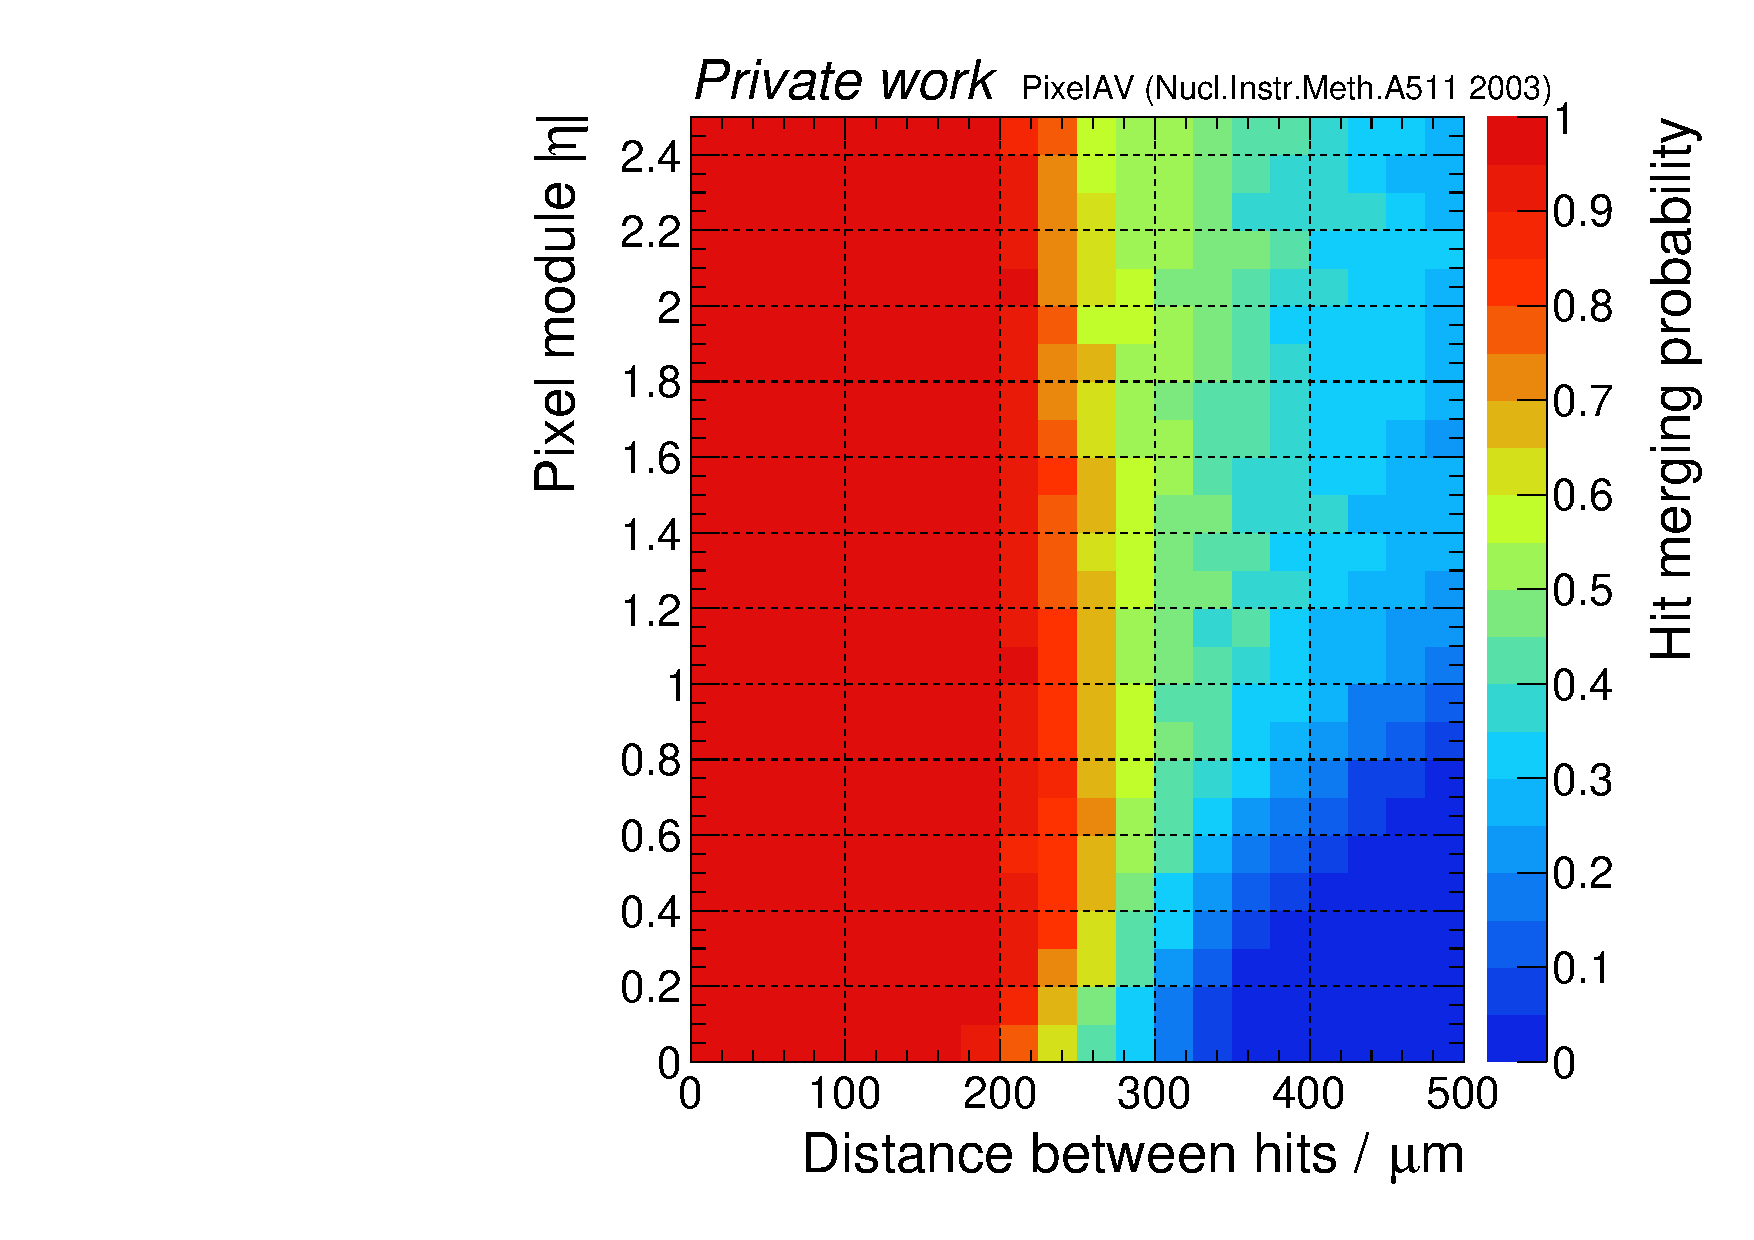
\includegraphics[width=0.4\textwidth]{figures/merge.pdf}
\caption{Probability of two hits merging on the pixel modules as a function of the distance and local incident angle expressed as pseudorapidity.}
\end{center}
\end{figure}

\section{Validation}

\begin{figure}[htbp]
\begin{center}
\parbox{0.46\textwidth}{\centering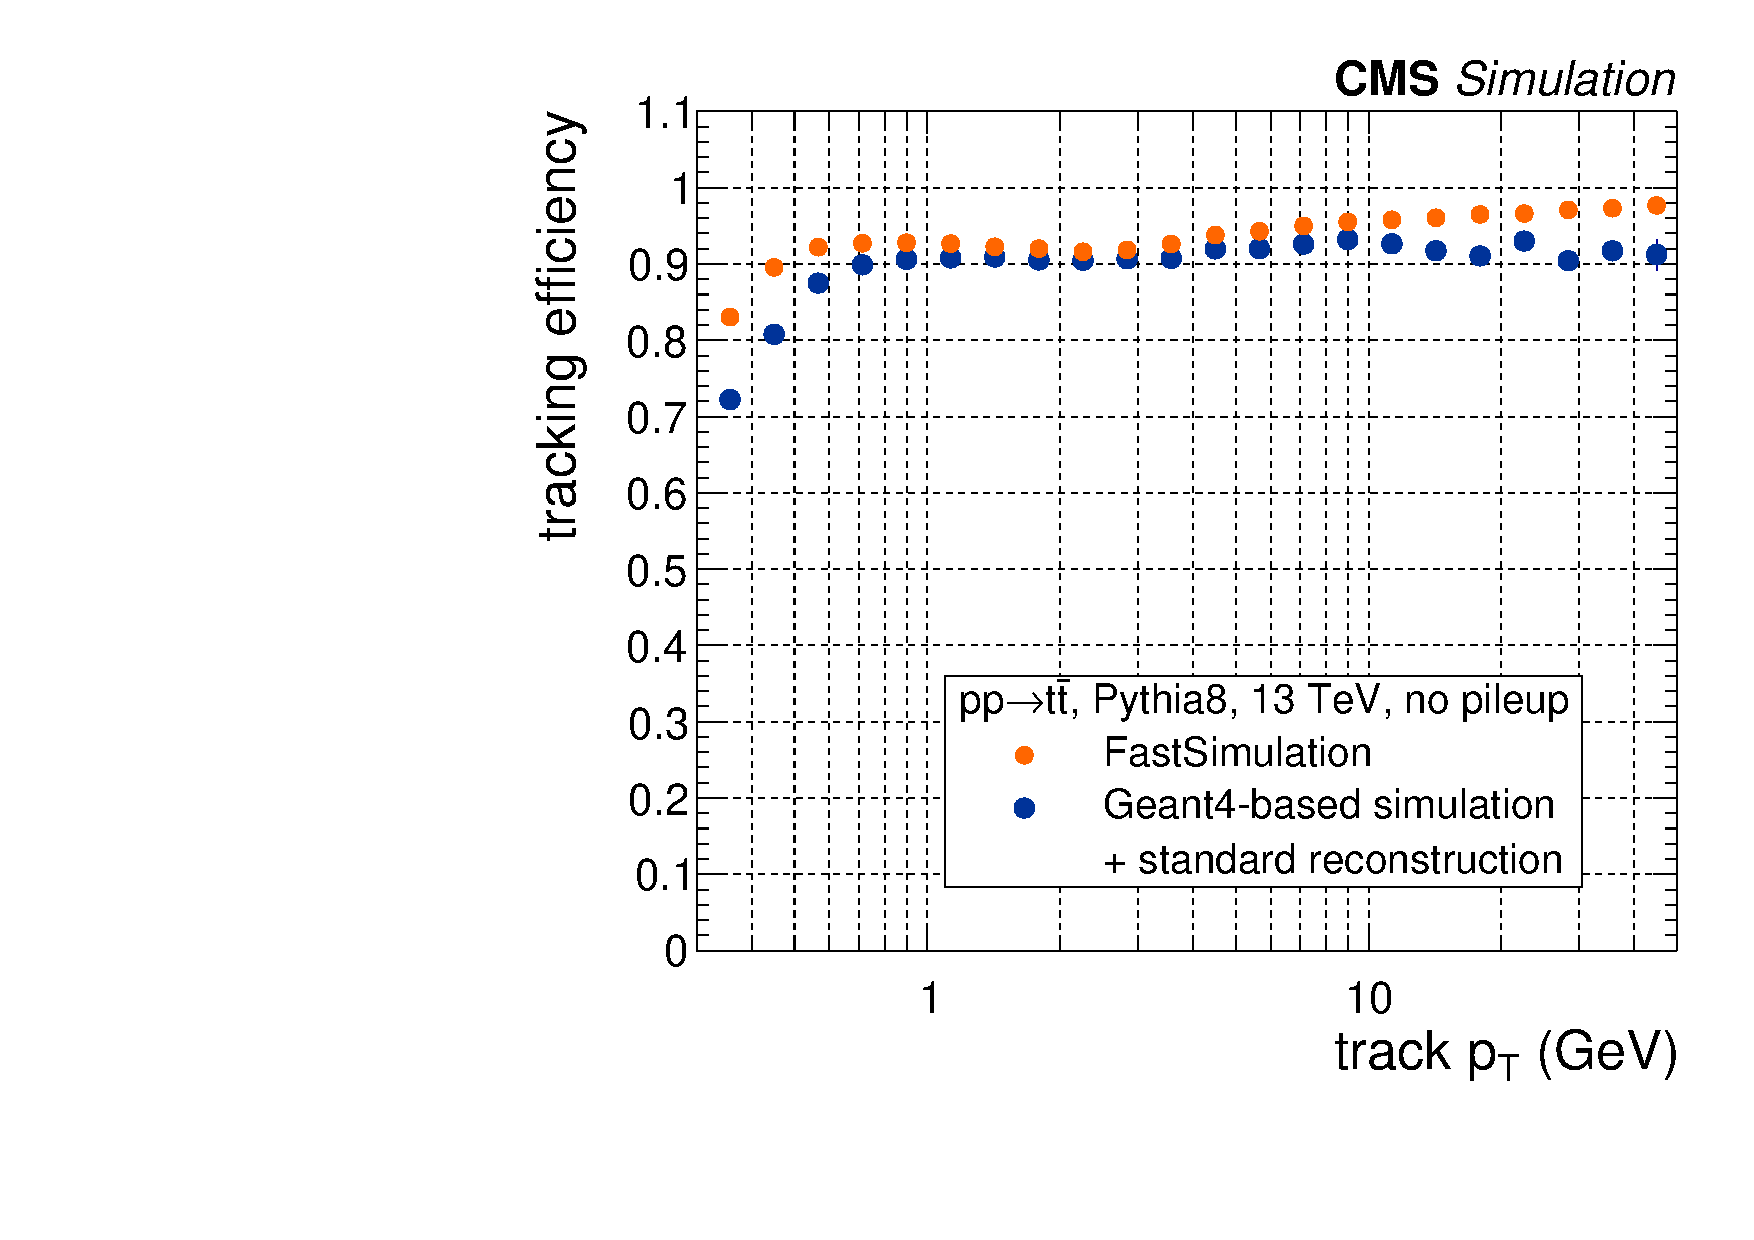
\includegraphics[width=0.45\textwidth]{figures/eff_pt.pdf}\\(a)}
\hspace{0.05\textwidth}
\parbox{0.46\textwidth}{\centering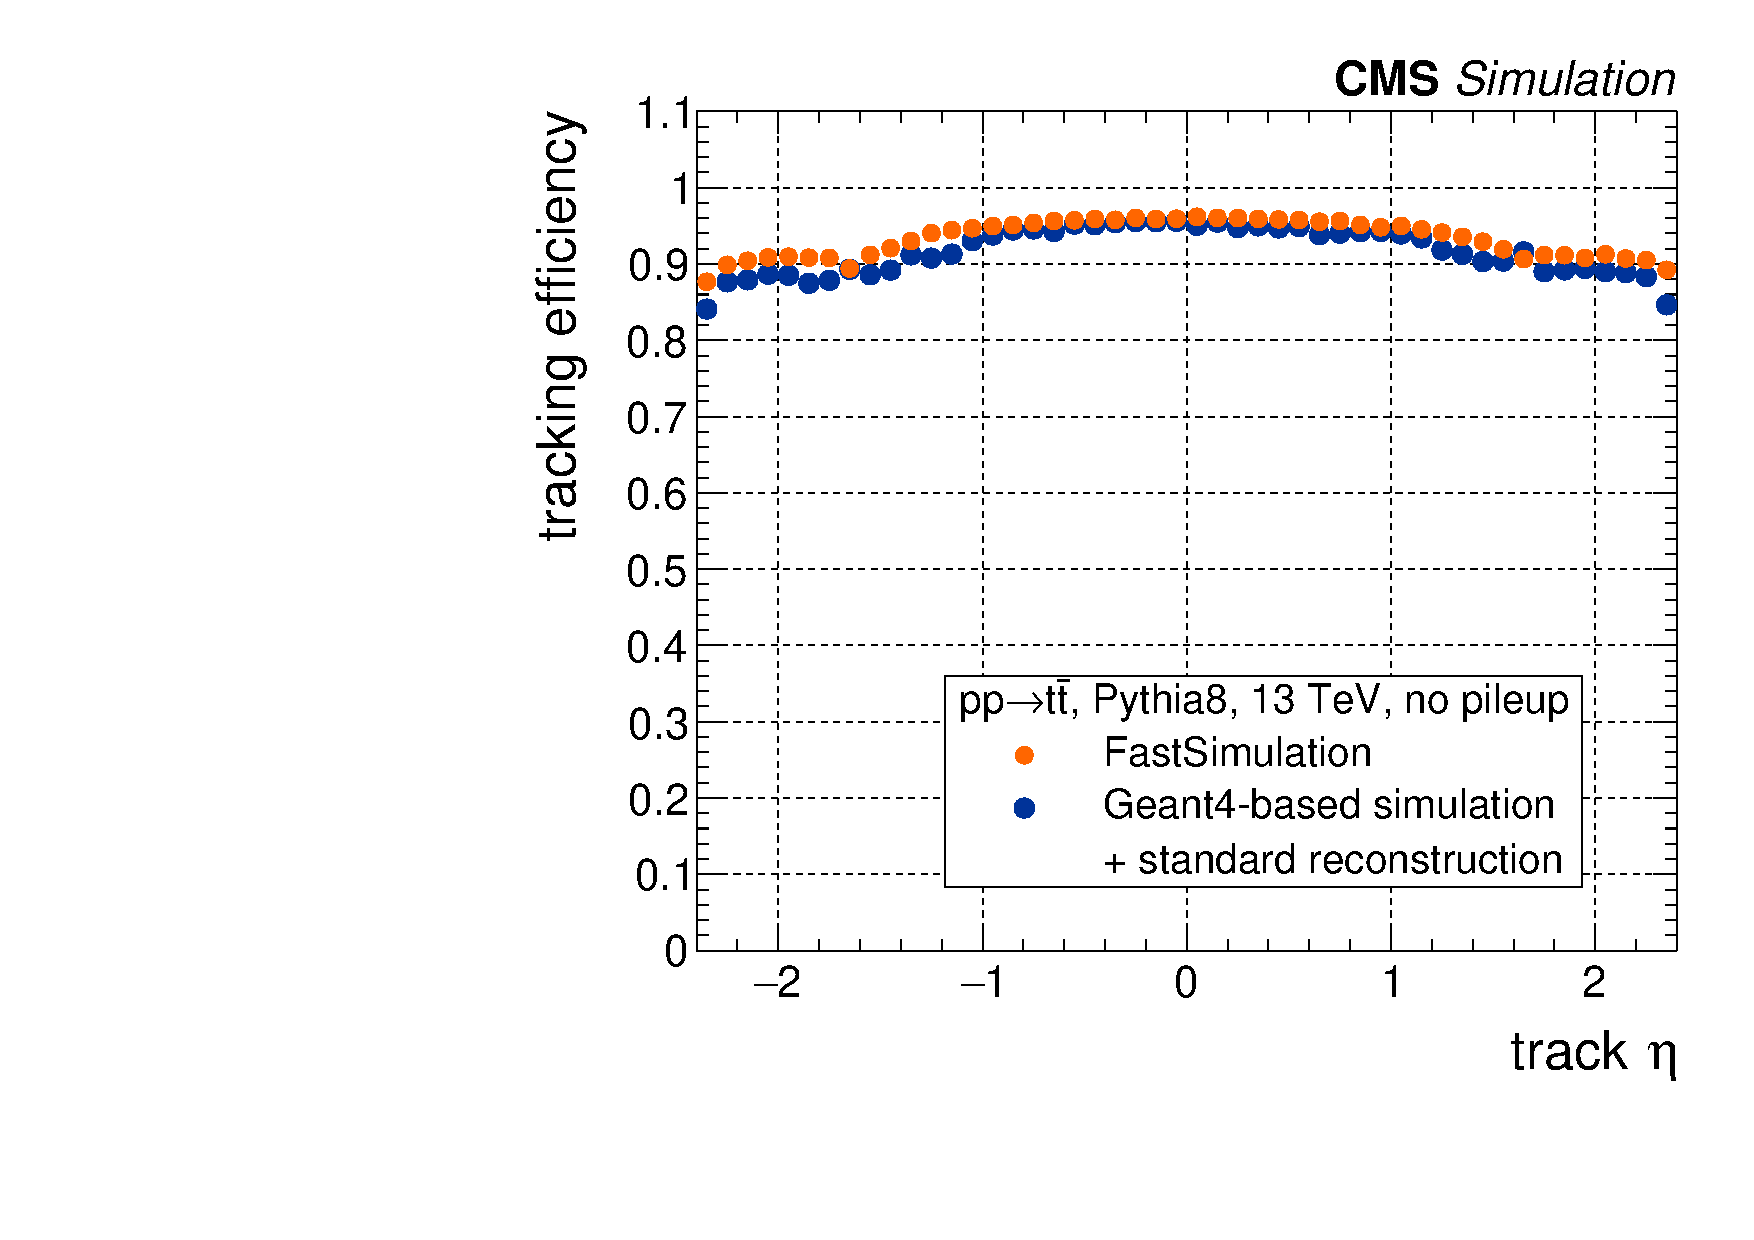
\includegraphics[width=0.45\textwidth]{figures/eff_eta.pdf}\\(b)}
\caption{Comparion of the reconstruction efficiencies of tracks as a function of (a)~the transverse momentum and (b)~the pseudorapidity.}
\end{center}
\end{figure}

\begin{figure}[htbp]
\begin{center}
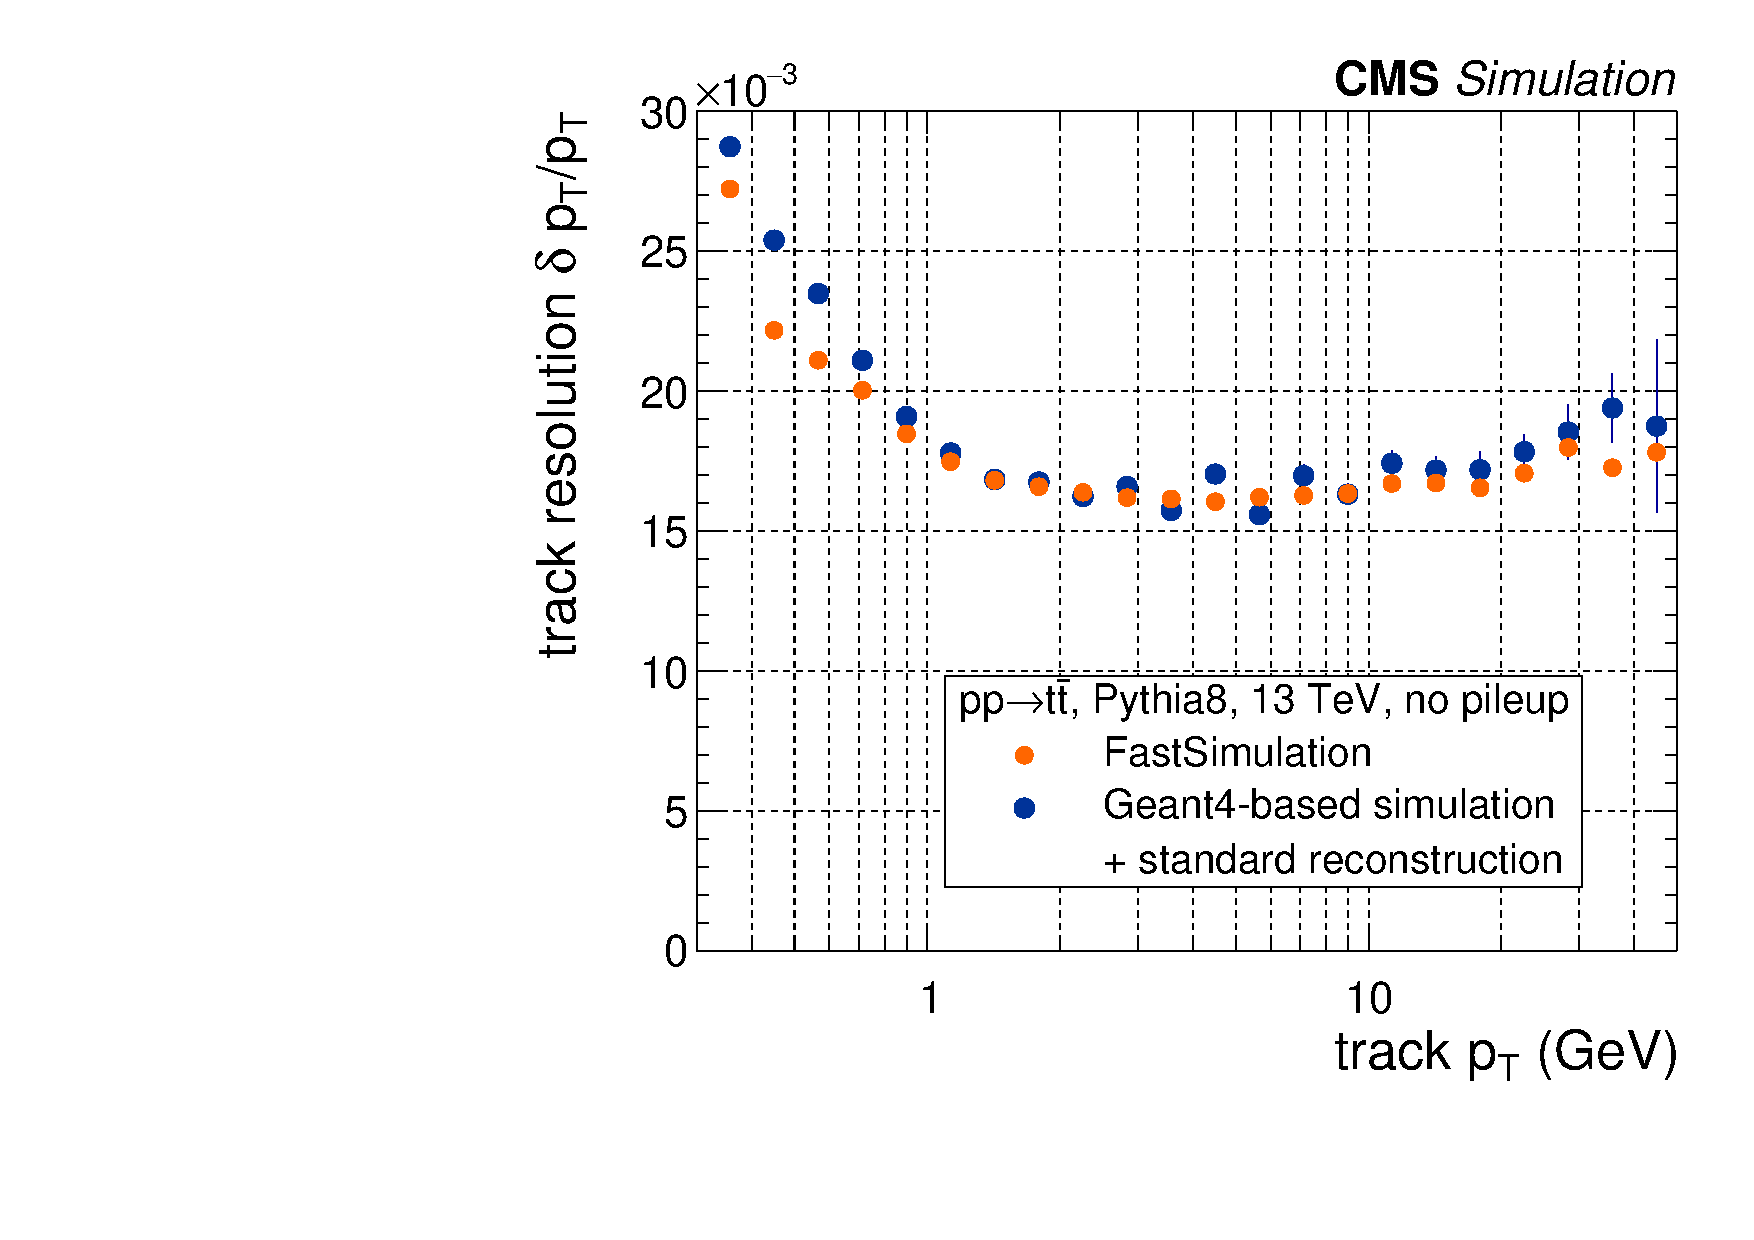
\includegraphics[width=0.45\textwidth]{figures/res_pt.pdf}
\caption{Comparion of the resolution of reconstructed tracks as a function of the transverse momentum.}
\end{center}
\end{figure}

\begin{figure}[htbp]
\begin{center}
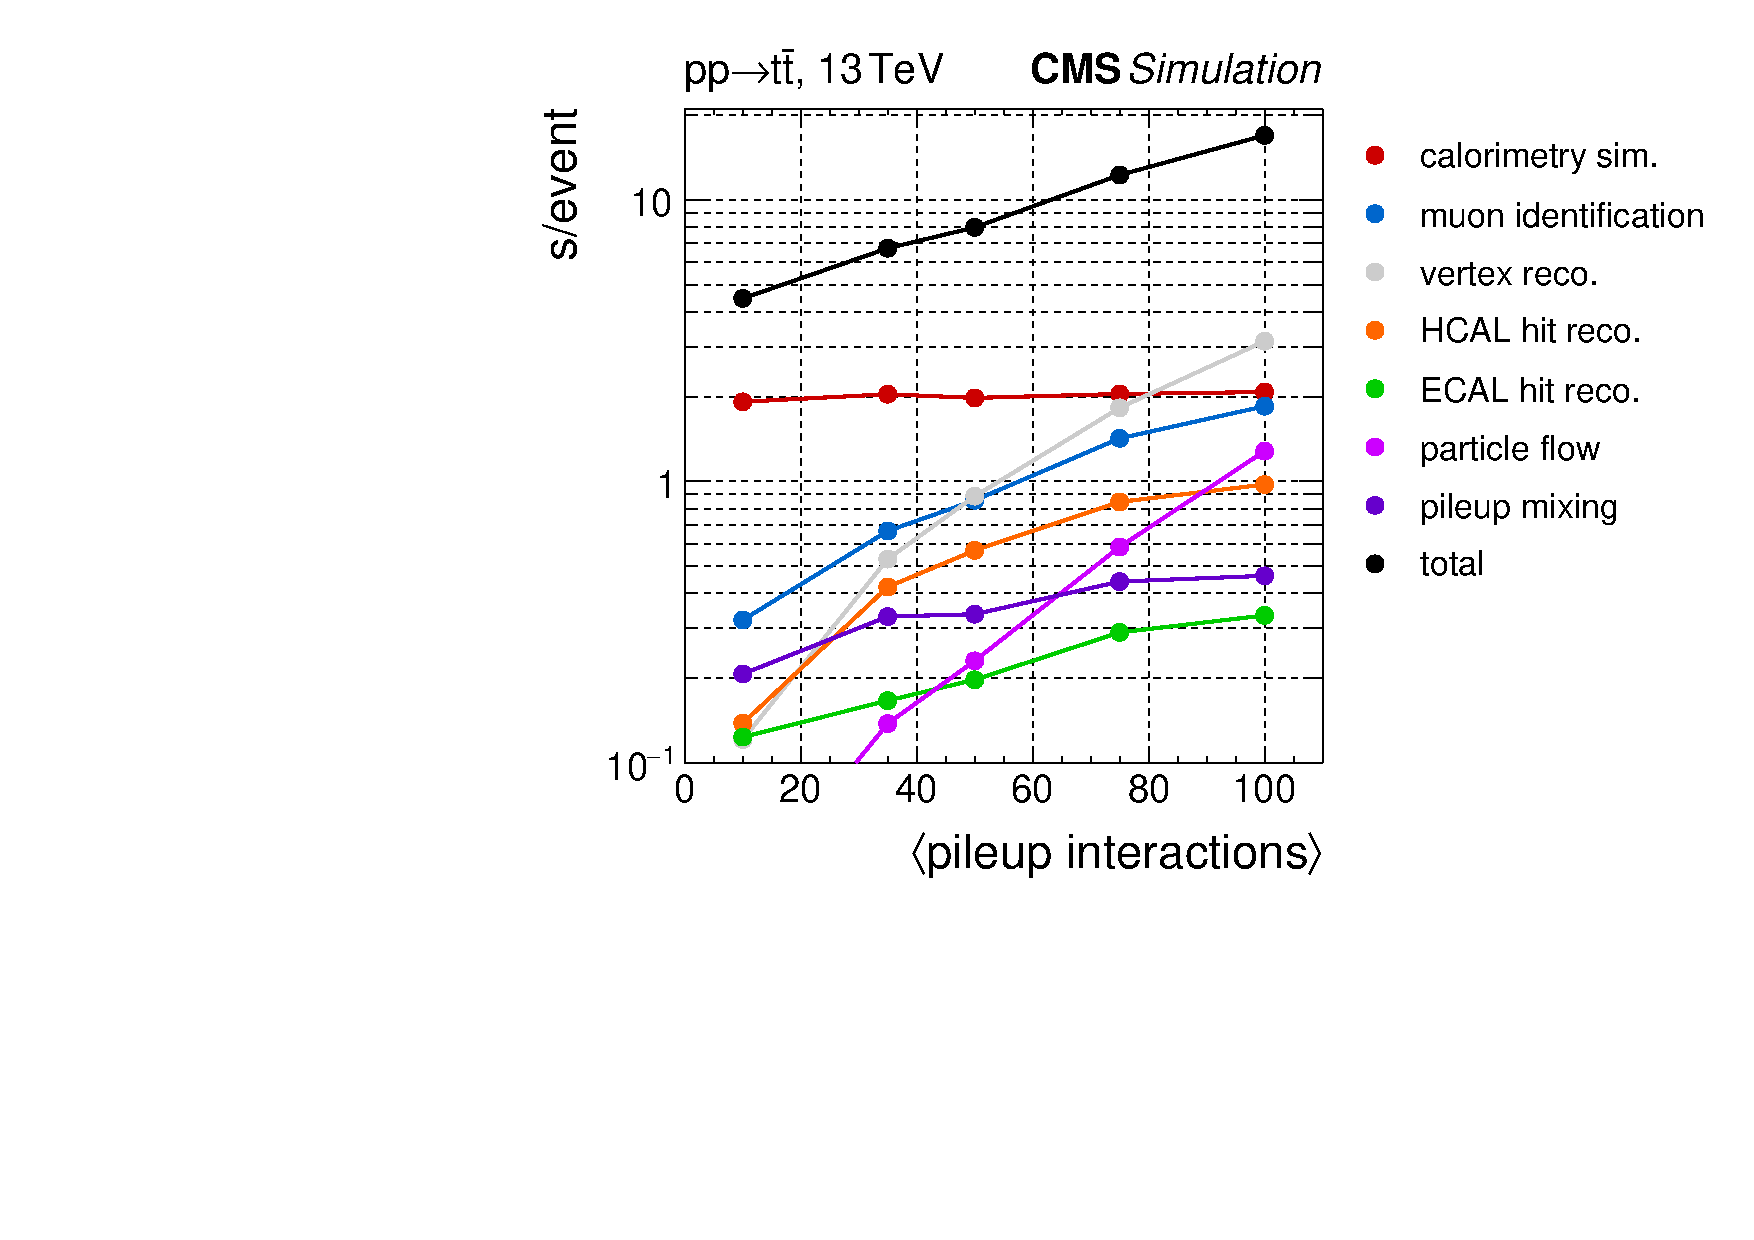
\includegraphics[width=0.55\textwidth]{figures/cpu_profile.pdf}
\caption{Average CPU-time per event for simulation and reconstruction within \textsc{FastSimulation} with as a function of the average number of pileup interactions.}
\end{center}
\end{figure}

\section{Summary and outlook}

\ack
The author thanks the organizers of the \textsc{CHEP2016} conference for the possibility of a poster presentation. Furthermore, funding is gratefully accepted from Fonds National de Recherche Scientifique~(FNRS), Belgium.


\section{References}

\begin{thebibliography}{9}
\item CMS Collaboration 2014, {\it JINST} \textbf{9} no.10, P10009.


%\item Strite S and Morkoc H 1992 {\it J. Vac. Sci. Technol.} B {\bf 10} 1237 
%\item Jain S C, Willander M, Narayan J and van Overstraeten R 2000 
%{\it J. Appl. Phys}. {\bf 87} 965 
%\item Nakamura S, Senoh M, Nagahama S, Iwase N, Yamada T, Matsushita T, Kiyoku H 
%and 	Sugimoto Y 1996 {\it Japan. J. Appl. Phys.} {\bf 35} L74 
%\item Akasaki I, Sota S, Sakai H, Tanaka T, Koike M and Amano H 1996 
%{\it Electron. Lett.} {\bf 32} 1105 
%\item O'Leary S K, Foutz B E, Shur M S, Bhapkar U V and Eastman L F 1998 
%{\it J. Appl. Phys.} {\bf 83} 826 
%\item Jenkins D W and Dow J D 1989 {\it Phys. Rev.} B {\bf 39} 3317 
\end{thebibliography}

\end{document}


